\documentclass[12pt,a4	]{report}
\usepackage[frenchb]{babel}
\usepackage[usenames,dvipsnames]{color}
\usepackage[utf8]{inputenc}
\usepackage{textcomp}
\usepackage[T1]{fontenc}
\usepackage{lmodern}	
\usepackage{bibunits}
\usepackage{graphicx}
\usepackage{wrapfig}
\usepackage{glossaries}
\usepackage{float}
\usepackage{cite}
\usepackage{caption}
\usepackage{amsmath,mathtools}
\usepackage{subcaption}

\begin{document}
\section*{Contribution}
\subsection*{Ouverture}
\paragraph{}
Les articles de Wikipédia sont constitués généralement du texte, mais aussi de certaines informations structurées (Infobox, images, liens externes, redirections entre les pages etc...) sous la forme de balises Wiki. 
Le projet DBpedia extrait des informations structurées de Wikipédia et les transforme dans une base de connaissances riche sous forme d'un graphe avec des entités reliées.
\subparagraph{}
Dans ce chapitre, nous allons vous donné une vue d'ensemble sur l'annotations des métadonnées, une analyse des besoins et la procédure d'extraction de DBpedia et les pistes de travail possibles. Puis nous présentons l'architecture globale de notre système, notre hypothèse et structure de notre application. 
\subsection*{Utilité des annotations}
\paragraph{}
En générale, l'annotation c'est ``quelque chose'' qu'on ajoute à une ressource Web. Depuis l'existence du Web, plusieurs système d'annotation du Web sont apparus (ThirdVoice, PageSeeder, HyperNews, Nestor, etc...).
Parmis les conséquences liées à ces systèmes d'annotation : l'information annotée doit d'une manière ou d'une autre être structurée ``utilisable'' et descriptive de la ressource ou de son utilisation ; la ressource en question doit exister et peut être exploitée sur le Web indépendamment des informations qui lui sont associées.
\begin{figure}[H]
\centering
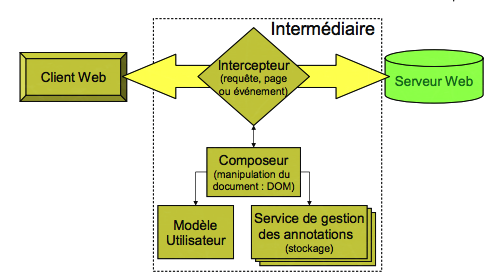
\includegraphics[width=9cm]{AnnotationSys.png}
\caption{Notation d'intermédiaire}
\end{figure}
\subparagraph{}
L'annotation sémantique fait référence à plusieurs types distinct d'annotations : formelles, explicites et permanentes. Il existe des outils d'annotation basées sur les ontologies {\it Ontology based annotation tool}.
Nous avons trouvé plusieurs critères relatives aux annotaions et liées aux systèmes par exemple : les types de resources concernées, structuration plus au moins forte des schémas de description, l'automatisation plus au moins marquée de la mise en place, etc...
\begin{figure}[H]
\centering
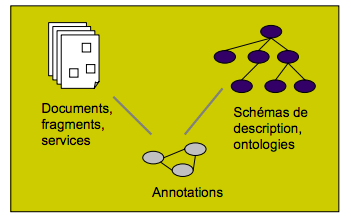
\includegraphics[width=9cm]{diffConnaissances.png}
\caption{Différents niveaux de connaissances}
\end{figure}
\subparagraph{}
L'annotation d'un triplet RDF est une façon d'ajouter des metadonnées à un triplet RDF pour décrire la validité temporelle, une restriction spatiale, ect...
\newline
\textit{Comment on utilise les annotations temporelles ? Exemple d'utilisation}
\subparagraph{}
Sur le site ``sig.ma''\footnote{http://sig.ma/} créer par \textit{the digital enterprise research institute in Ireland}, la plateforme fournit un moteur de recherche par mot clé qui permet de récupérer des images et des textes accessibles par des annotations RDF, ainsi que d'une liste d'URI synonymes correspondant à la clé de recherche et des liens vers des sources Web contenant des données RDF pertinentes.
\subsection*{Analyse des Besoins}
\paragraph{}
Le large succès de Wikipedia (qui est le 2éme site le plus visité sur internet) et le progrès des techniques d’extraction des données ont abouti à la naissance de la construction automatique  de larges base de connaissances comme DBpedia, YAGO, etc...
\subparagraph{}
Beaucoup de connaissances sont construites en se basant sur l’extraction automatique des faits relationnels dans un texte.
Malheureusement, les bases de connaissances convergent sur les faits statiques et ne donnent pas une grande importance à la dimension temporelle de ces faits.
Malgré le fait que la majorité des faits évoluent avec le temps, ou n'est valide que dans une période temporelle précise. Ainsi, nous remarquons que le temps a une dimension significatif dans ces bases de connaissances.
\subparagraph{}
La dimension temporelle est particulièrement importante dans les relations binaires comme $isPresidentOf$, $isCEOof$, $isMarriedTo$, on peut être mariée à plusieurs épouses mais dans des différents intervalles de temps mais ``On ne prend pas compte des exceptions de mariage polygames''.
\subparagraph{}
Une base de connaissances contenant plusieurs présidents des États-Unis ne peut être consistante que lorsqu’on ajoute une dimension temporelle à ces faits. De plus l’annotation temporelle aide à faire la distinction entre les faits courants et les faits dépassés.
Par exemple le fait ``Kennedy est le président des États-Unis'' est correct, mais n'est plus valide.
Lorsqu’on attache une annotation temporelle à un fait comme celui là, il devient universellement valide.
\begin{figure}[H]
\centering
\includegraphics[width=10cm]{Sources.png}
\caption{Différentes sources d'informations dans DBpedia}
\end{figure}
\subsection*{Problèmatique}
\paragraph{}
Lorsqu’on parcourt DBpedia, on trouve beaucoup de triplets qui décrivent des informations temporelles. Ces derniers sont généralement liées à un contexte événementiel précis.
Il est plus difficile d’exploiter ces informations si elles ne possèdent pas une structure claire et lisible par la machine.
\newline
Dans DBpedia, il se trouve que des informations liées au même contexte temporel sont exprimées de la manière suivante: 
\begin{figure}[H]
        \centering
                \centering
                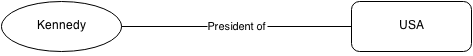
\includegraphics[width=10cm]{ken.png}
               \caption{triplet ''Kennedy''}

\end{figure}
\subparagraph{}
Le premier triplet n'a pas une sémantique valide que en tenant compte du triplet suivant~: 
\begin{figure}[H]
        \centering
                \centering
                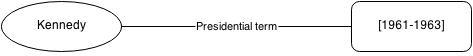
\includegraphics[width=10cm]{presidterm.png}
               \caption{triplet presidential term ''Kennedy''}

\end{figure}
\subparagraph{}
On vise plutôt à annoter les triplets ($s$, $p$, $o$) avec une étiquette temporelle qui précise la validité de ce terme dans un cadre logique qui appartient au monde réel où en dehors de ce cadre, on peut dire que ce triplet RDF n’est pas valide et qu’on ne peut pas l’utiliser.

\subsection*{Étude préliminaire et approches possibles}
\subsubsection*{Web Collaboratif}
\paragraph{}
C'est le Web qui s'appuie sur les utilisateurs pour construire son contenu. Nous avons commencé notre travail de recherche avec une première approche ; nous avons étudié les pistes possibles pour l'exploitation des dumps de Wikipédia et Wikidata. Tout d'abord, nous avons téléchargé les fichiers des collections XML et nous avons commencé par l'implémentation d'un algorithme d'extraction avec un parseur SAX\footnote{http://fr.wikipedia.org/wiki/Simple\_API\_for\_XML}.
La figure ci-dessous présente notre schèma de modélisation dans lequel nous avons procédé avec une modélisation qui touche directement la source principale d'informations Wikipédia.
\begin{figure}[H]
        \centering
                \centering
                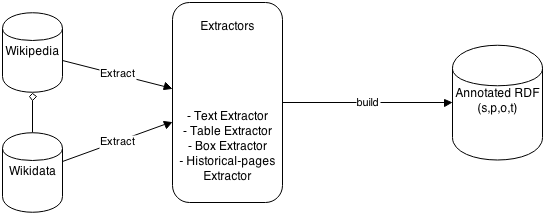
\includegraphics[width=10cm]{modelisation.png}
               \caption{Première approche : schéma de modélisation générale}

\end{figure}
\subsubsection*{Traitement automatique des langues}
\paragraph{}
Le traitement automatique de la langue (TAL) est une dicipline à la frontière linguistique liée à l'intelligence artificielle.
Il existait un type de TAL statistique proposent des méthodes statistiques, probabilistes ou purement statistiques pour résoudre pour résoudre certaines difficultés.
On distingue plusieurs domaine d'application de TAL : traduction automatique, génération automatique de texte, correction orthographique, reconnaissance de l'écriture manuscrites etc...
Mais dans ce type de traitement il y a pas mal de problème qui peuvent apparaître et principalement celui de l'ambiguïté temprelle.

\subsubsection*{Ambiguïtés temporelles}
\paragraph{}
C'est la propriété d'un mot ou d'une suite de mot (comme notre cas) qui peuvent sens ou plusieurs analyses grammaticales possible. Dans une phrase simple ou composée l'indicateur temporel peut avoir plusieurs sens tout dépend du contexte de la phrase.
\newline
Les informations temporelles peuvent avoir des repèsentations différentes~: 
\begin{itemize}
\item Un évènement ``Je vous propose un rendez-vous $demain$ pour parler de ma plateforme PiSharing''. \item Une connaissance ``Jacques Chirac est le président de la république Française'' \textbf{ mais quand ?}.
\end{itemize}

\subparagraph{} 
Le présent par exemple peut avoir plusieurs sens ou contextes : présent de narration, présent de généralité, présent qui réfère au futur proche, etc...
Les signaux temporelles sont ambigus par exemple dans ces expressions : il court pour rattraper le temps, tu tournes après la rivière, etc…, on remarque qu'il y a des indicateurs temporelle mais ce n'est pas le temps qui est relative à un événement qui peut nous intéresse.
La plupart des expressions sont floues comme: il y a deux ans, chaque deux semaines, j’arrive dans deux secondes, etc..., il n'y a pas une logique descriptive qui peuvent nous aider à mettre un le lien entre l'évément et la période temporelle.
\paragraph{}
L’analyse du temps s’inscrit dans la compréhension globale des textes, et des évènements auxquels on fait référence dans ce texte non pas en analysant une phrase comme suit. 
\newline
Modalité~: ``l’équipe de France voulait gagner la coupe du monde en 2006.'' 
\newline
Anaphore~:  ``..., cela pourrait avoir lieu dans les éditions suivantes.''
\subparagraph{}
Les évènements décrits (et que l’on souhaite fixer temporellement) peuvent être: duratifs ou ponctuels/accomplis ou inaccomplis. 
De même pour les dates qui peuvent être des dates absolues ``le 18 mars, c'est mon anniversaire''; ou bien des dates relatives par rapport au moment de l’énonciation par exemple : `` il y a deux ans''. Pour la durée aussi on distingue plusieurs type comme la durée absolue `` durant 2 ans'' et la durée relative~: `` depuis un an''. Dans un texte on trouve aussi un ensemble d'expressions de fréquence par exemple ``tous les ans, le vendredi 13'' et des expressions plus complexes comme ``après la Révolution Tunisienne''.
\subparagraph{}
Les textes contiennent des informations temporelles de taille massive qui sont difficilement exploitable. Nous avons essayé de donner une vue globale sur cette procédure que nous avons décidé de ne pas l'adopter parce que notre objectif est d'annoté des triplets RDF plutôt que de faire l'analyse des textes. Nous détaillerons par la suite l'architecture de DBpedia à partir de laquelle on s'inspire pour proposer notre solution.
\subsubsection*{Historique des modifications dans Wikipédia}

\paragraph{}
C'est une page attacher à un article encyclopédique pour concerver le journal de la plupart des modifications qui ont été apportées à cet article. L'historique d'une page permet de connaître la date, l'auteur et la teneur externe de chaque modification 
Nous avons remarqué qu'appartir de l'historique de modifications dans cette encyclopédie on peut déduire plusieurs informations liée à deux ou plusieurs context temporel différent.
Nous souhaitons, si c’est possible, extraire ces informations temporelles. Car, il se trouve qu’il y en a beaucoup d’informations liées à cet historique.
\begin{figure}[H]
\centering
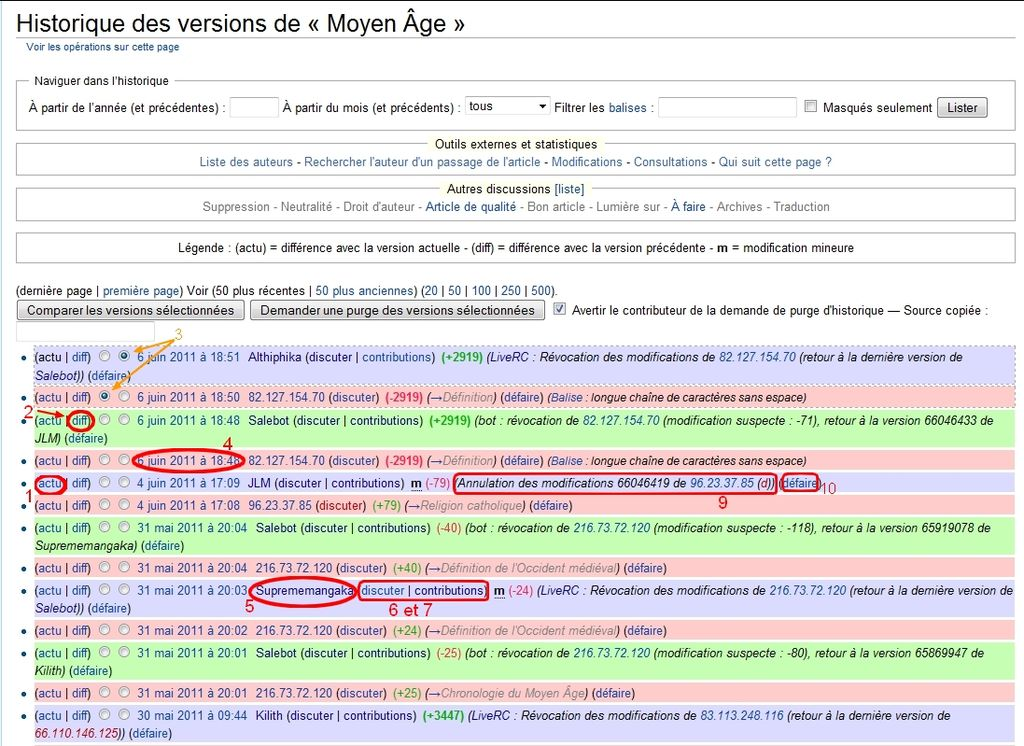
\includegraphics[width=6cm]{Historique_articles.jpg}
\caption{Historique d'articles Wikipédia}
\end{figure}
\newpage

\subsection*{Architecture d'extraction de DBpedia}
\begin{figure}[H]
\centering
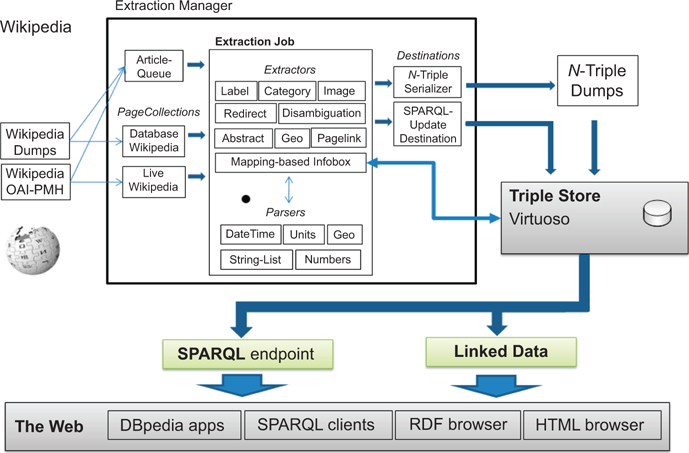
\includegraphics[width=12cm]{dbpediaExtra.png}
\caption{Extracteur DBpedia}
\end{figure}
La figure ci-dessus montre l'architecture du système d'extraction des connaissances dans DBpedia.
D'apres Morsey et al~\cite{morsey2012} les principaux éléments du système sont les suivants : $PageCollections$ est une abstraction des ressources locales ou distantes des articles de Wikipédia, $Collections$ stokent ou sérialisent les triplets RDF extraite, $Extractors$ qui transforme un type spécifique de la syntaxe wiki en triplet, $Parsers$ soutiennent les $Extractors$ en déterminant les types de données, convertit les valeurs entre différentes unités et fractionne les marqueurs dans des listes. L'$Extraction$ $Job$ regroupe une collection de pages, extracteurs et destination dans le flux de travail $workflow$.
Le noyau de ce système est l'$Extraction$ $Manager$ qui gère le processus  d'adoption des articles de Wikipédia sur les $Extractors$ et donne les résultats à la destination.
Le gestionnaire d'extraction $Extraction$ $Manager$ gère également la gestion des URI et résout les redirections entre les articles : ce système se compose de $11$ extracteurs qui traitent les types des contenus de Wikipédia ($Labels$, $Abstracts$, $Interlanguage$ $links$, $Images$, $Redirects$, $Disambiguation$,
$External$ $Links$, $Pagelinks$, $Homepages$, $Categories$, $Geo-coordinates$).
Ce framework d'extraction DBpedia est mise en place pour réaliser deux flux : extraction à partir des dumps ($DataBaseWikipedia$ $page$ $collections$) et une procédure d'extraction direct
($LiveWikipedia$ $page$ $collections$ $with$ $the$ $OAI-PMH$ $protocol$) pour obtenir la version courante des articles.
\subsection*{Notre modélisation}
\paragraph{}
Le modèle quaternaire est un modèle qui capte la base du fait avec un indice temporel, l'exemple suivant montre le principe de ce modèle.
\newline
{\it <politician> elected <president of US> on <date>}
\newline
f1, Kennedy elected PresidentOfUSA 
\newline
f2:f1, HappenedDate
\newline
{\it <politician> served as <politician office> from <date> to <date>}
\newline
f1, Kennedy holdsPoliticalPosition PresidentOfUSA 
\newline
f2:f1, startedOnDate 
\newline
f3:f1, endedOnDate
\newline
$HappenedDate$ est utilisée pour dire que le fait est valide que dans ce point du temps.
\begin{figure}[H]
        \centering
                \centering
                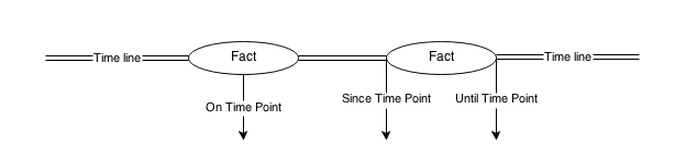
\includegraphics[width=10cm]{timeline.png}
               \caption{Chronologie des événements}

\end{figure}
\subparagraph{}
Pour surmonter ce problème et exprimer la validité temporelle d’un triplet RDF d’une manière à la fois intelligente et lisible par la machine; on souhaite rattacher au triplets valides que dans un point du temps ou une plage temporelle bien précise une étiquette temporelle adéquate comme le montre la figure suivante.
\begin{figure}[H]
        \centering
                \centering
                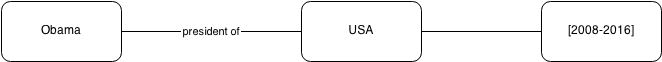
\includegraphics[width=10cm]{obamaQuad.png}
               \caption{Modélisation quadruplet}

\end{figure}
\subparagraph{}
On s'intéresse particulièrement au format N-Quads comme format de sortie de notre algorithme. Les quadruplets vont être formalisés de la manière suivante~:
\newline
$<s,p,o,t>$ : un sujet, prédicat, objet avec un point de temps.
\newline
$<s,p,o,[t1,t2]>$ : de même avec une intervalle de temps.


\subsubsection*{Résumé}

Dans cette section, nous avons présenté notre approche dans le but est de mettre en place un système d'annotation temporelle des triplets dans DBpedia. Dans un premier, lieu nous avons effectué une étude préliminaire en analysant les besoins et en étudiant l'architecture de la base de connaissance.
Par la suiter une deuxième solution que nous avons trouvé plus intéressante et que nous avons implèmeneté  sous forme d'un prototype fonctionnel.
\paragraph{}
\bibliography{Biblio.bib}
\end{document}